\documentclass{article}

% if you need to pass options to natbib, use, e.g.:
% \PassOptionsToPackage{numbers, compress}{natbib}
% before loading nips_2017
%
% to avoid loading the natbib package, add option nonatbib:
% \usepackage[nonatbib]{nips_2017}

\usepackage[final]{nips_2017}

% to compile a camera-ready version, add the [final] option, e.g.:
% \usepackage[final]{nips_2017}

\usepackage[utf8]{inputenc} % allow utf-8 input
\usepackage[T1]{fontenc}    % use 8-bit T1 fonts
\usepackage{hyperref}       % hyperlinks
\usepackage{url}            % simple URL typesetting
\usepackage{booktabs}       % professional-quality tables
\usepackage{amsfonts}       % blackboard math symbols
\usepackage{nicefrac}       % compact symbols for 1/2, etc.
\usepackage{microtype}      % microtypography
\usepackage{graphicx}
\usepackage{caption}

\title{Machine Learning Project - Stock Fluctuations}

\author{
  Mary Letey \\
  \And
  Morgan Allen \\
  \And
  Colton Williams \\
  \And
  Aniq Shahid 
}

\begin{document}

\maketitle

\begin{abstract}
  Research project investigating relationships between media concerning companies and the aforementioned company's stock price. Theoretically, the stock price of a company is based in part on public perception of their market. This perception can easily be affected by media sources, such as news sources and Google trends. \textbf{TODO :: One sentence on results}. An extension of this project would be to include Twitter data as a form of public perception. 
\end{abstract}
 
\section{Introduction}

Stock prices seem unpredictable; however, \emph{theoretically} they are quite simple. Considering the most basic supply-demand model in economics, stock prices are functions of the supply and demand for ownership in a company. A company's stock price depends heavily on the investors' perception of the company, such as perceived growth and perceived risk. In other words, because the "consumers" in this model are viewing a stock as an investment, demand represents confidence in the performance of the company. Furthermore, an increasing stock price represents increased confidence in the potential of the company. Thus the stock price can be affected by a change in the public's perception of a company's risk. Forms of media, such as news articles, can have a huge impact in these perceptions.

\begin{figure}[h]
    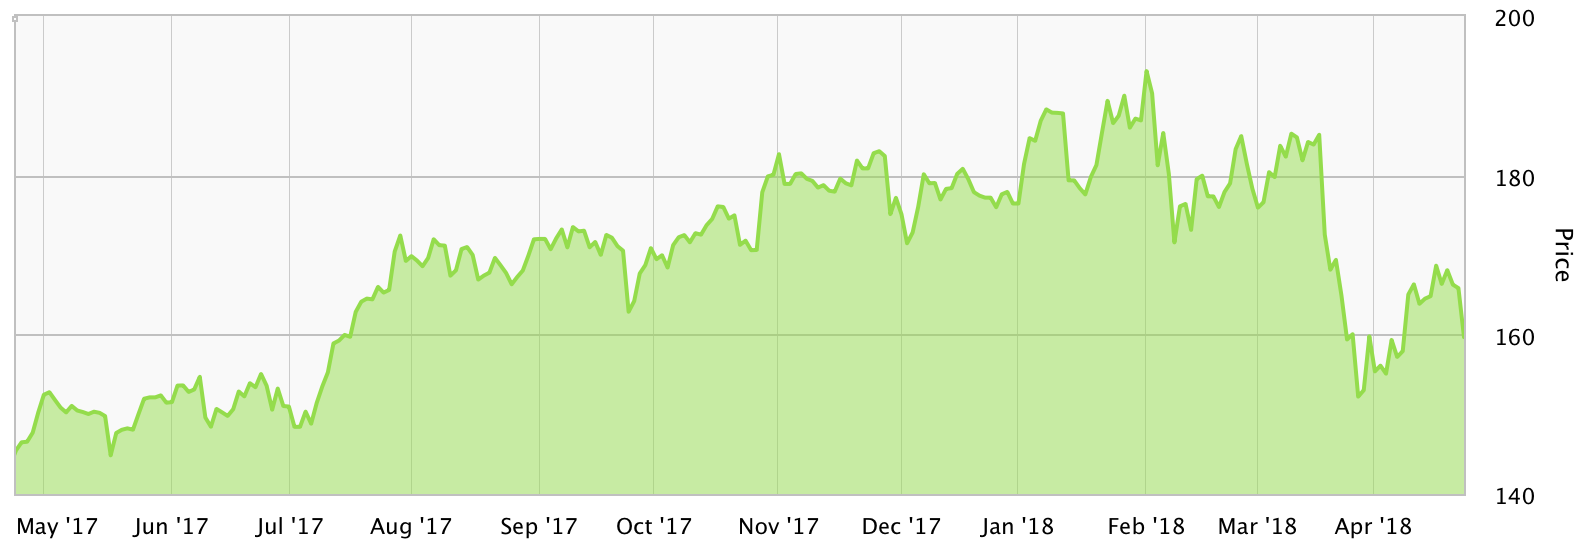
\includegraphics[scale=0.5]{FacebookYear.png}
  \caption{Facebook's stock price over the last year}
  \label{fig:faceplant}
\end{figure}

For example, when examining Facebook's stock price over the last year, one of the most prominent features in Figure \ref{fig:faceplant} is the dramatic drop around the beginning of April. Recall, Mark Zuckerburg testified before congress on April 8th. This hearing caused concern about Facebook's future, where traders expected Facebook's stock price to continue declining around a window of April 8th, according to Business Insider [1].

This project will examine the extent to which media sources affect stock prices, and how well we can use media data to predict stock price changes. 

\newpage 

\section{Data and Methods}

The focus of this project is to investigate the effects of media on stock price changes inside the technology industry. A single industry was chosen in order to maintain consistent results. The companies in this project representing the tech industry are: \begin{itemize}
\item Hewlett Packard
\item IBM
\item Seagate
\item Western Digital
\item \textbf{TODO :: replacement for Dell here}
\end{itemize}

The focus of the media data is incorporating textual data from news articles into our model. The articles were gathered from reputable news sources such as the Wall Street Journal. 

Furthermore, data from Google Trends is also included to obtain correlation between certain terms to model public interest in the company.  

Numerical data measuring the closing price and volatility of shares was retrieved from Bloomberg. Other numerical data included macro-economic factors, such as the S\&P500, crude oil, and gold. 

\section{Results and Discussion}

The Google Trends data provided an excellent starting point for this analysis. As one would expect, given that they measure public interest in a company, the Google Trends data combined with previous stock data predicted the closing price of the company's shares. 
\begin{figure}[h]
	\centering
    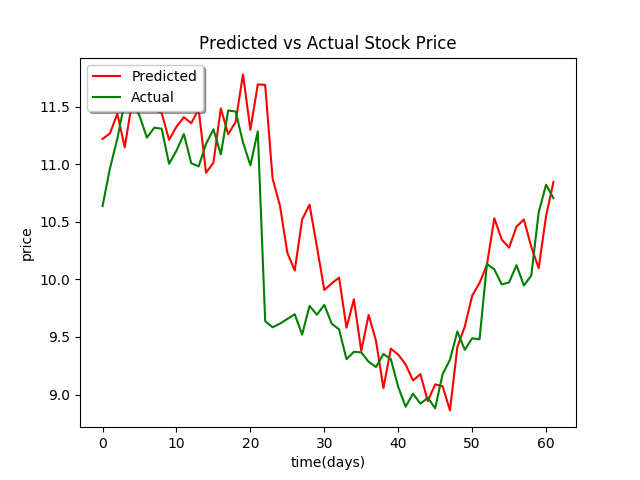
\includegraphics[scale=0.65]{googleHP.png}
  \caption{Using Google Trends to Predict Closing Price}
  \label{fig:googlehp}
\end{figure}

For example, Figure \ref{fig:googlehp} shows almost exact results using a standard regression, where the Predicted and Actual curves are almost completely correlated. 

\section{Conclusions}

\section{References}

\small

[1] Ciolli, Joe (2018, April 10) \emph{Facebook traders are bracing for the worst ahead of Mark Zuckerberg's hearing}. Retrieved from \url{http://www.businessinsider.com/facebook-stock-price-hedging-ahead-of-mark-zuckerberg-congressional-testimony-hearing-2018-4}

\end{document}
